\documentclass{proposalnsf}
\usepackage{epsfig}
\usepackage{hyperref}
\usepackage{booktabs}
\usepackage{graphicx}
\usepackage{wrapfig}
\usepackage{float}
\restylefloat{table}

% NSF proposal generation template style file.
% based on latex stylefiles  written by Stefan Llewellyn Smith and
% Sarah Gille, with contributions from other collaborators.

\newcommand{\jas}{{\it J. Atmos. Sci.}}
\newcommand{\jpo}{{\it J. Phys. Oceanogr.}}
\newcommand{\JPO}{{\it J. Phys. Oceanogr.}}
\newcommand{\jfm}{{\it J. Fluid Mech.}}
\newcommand{\jgr}{{\it J. Geophys. Res.}}
\newcommand{\JGR}{{\it J. Geophys. Res.}}
\newcommand{\jmr}{{\it J. Mar. Res.}}
\newcommand{\arfm}{{\it Ann. Rev. Fluid Mech.}}
\newcommand{\dsr}{{\it Deep-Sea Res.}}
\newcommand{\dao}{{\it Dyn. Atmos. Oceans}}
\newcommand{\jam}{{\it Journal of Applied Meteorology}}
\newcommand{\phfl}{{\it Phys. Fluids}}
\newcommand{\phfla}{{\it Phys. Fluids A}}
\newcommand{\PhilTrans}{{\it Philosophical Transactions of the Royal Society, 
London}}
\newcommand{\gafd}{{\it Geophys. Astrophys. Fluid Dyn.}}
\newcommand{\gfd}{{\it Geophys. Fluid Dyn.}}
\newcommand{\PCE}   {{\it Physics and Chemistry of the Earth}}
\newcommand{\PRL}   {{\it Physical Review Letters}}

\newcommand{\ProgOc}{{\it Prog. Oceanography}}
\newcommand{\WHOITR}{Woods Hole Oceanographic Institution Technical Report, WHOI-}
\newcommand{\degrees}{$\!\!$\char23$\!$}
%%% old lines below defined some mathematical fonts; these no longer seem necessary
%\DeclareFontFamily{OT1}{psyr}{}
%\DeclareFontShape{OT1}{psyr}{m}{n}{<-> psyr}{}
%\def\times{{\fontfamily{psyr}\selectfont\char180}}


\renewcommand{\refname}{\centerline{References cited}}

% this handles hanging indents for publications
\def\rrr#1\\{\par
\medskip\hbox{\vbox{\parindent=2em\hsize=6.12in
\hangindent=4em\hangafter=1#1}}}

\def\baselinestretch{1}

\begin{document}


\noindent{\Large{\bf Computational Modeling to Aid in Analysis and Interpretation of Multi-Modal Neutron Experiments }}\\*[3mm]

\pagenumbering{arabic}
\renewcommand{\thepage} {\arabic{page}}



\section*{Research Objectives}
The over-arching goal of our project is to create a streamlined workflow
for experimental data analysis and interpretation
needs of the neutron scattering community using atomistic modeling and
simulation. Neutron scattering experiments require users to model and
interpret data at the atomic level. With numerous software
applications and a large array of different file formats with each,
scientists tend to use a limited (and sometimes dated) subset of
software tools to tackle data analysis from neutron experiments. This
creates a barrier in their research between experimental and theoretical techniques.

We are currently developing a modeling and analysis workbench called the 
Integrated Computational Environment-Modeling \& Analysis for Neutrons,
or ICE-MAN. This is an extension of the Eclipse ICE project \cite{ICEwebsite}. We hope to create a seamless transition from both different
types of neutron scattering experimental data and computer modeling and
simulation techniques to tackle multi-modal data
analysis. An example of a workflow would be the study of a disordered
material. First, neutron scattering experiments could yield the average
structure of the material (diffraction data) and
the local structure via total scattering (the pair
distribution function, or PDF).  Molecular dynamics (MD) simulations can provide
a trajectory for an atomistic model  giving an
ensemble of possible atomic configurations to compare to experiment.
Sampled configurations from the trajectory could be used as inputs into reverse Monte Carlo modeling (RMC) to optimize the structures against the the diffraction and PDF data produced from the neutron scattering experiments.
The MD trajectories could also then be used to calculate the
inelastic neutron scattering spectrum of the system. This data could
feed back into the RMC modeling as a constraint. At present this process
would be exceedingly time consuming, involve expertise in multiple
techniques, and most likely present a barrier that would
seldom be overcome by general users.

We are requesting XSEDE's HPC resources to carry out this workflow on the outlined projects that already have a need for computational approaches to solve complex structural data analysis and also multiple potential projects for the general neutron scattering community, specifically Users of the Spallation Neutron Source (SNS) instruments at Oak Ridge National Lab. We propose three projects that have already been studied via neutron scattering experiments and have a need for atomistic modeling to aid in the data analysis process. These include irradiated amorphous silica for nuclear radiation damage on materials, high-pressure amorphous silica for cheaper manufacturing of electronics, and oxygen insertion into shafarzikite-like structures for oxygen storage materials.


\subsection*{Proposed Research}
\subsubsection*{Project 1: Investigate structural modifications of irradiated silica for nuclear materials}\label{lang}

The first project would be the study of the local structure changes in amorphous silica (SiO2) before and after irradiation of high energy
(tens of MeV or more) heavy ion bombardment, or swift heavy ions (SHIs). At these high energies, electronic stopping dominates over nuclear stopping, implying the SHI interacts with the electronic structure of the irradiated target material. The SHI path deposits energy to the electronic structure which then dissipates the energy to the nuclear motion of the material, causing a local heat spike in the material radially perpendicular to the SHI pathway. 

\begin{wrapfigure}{r}{0.5\textwidth}
  \begin{center}
    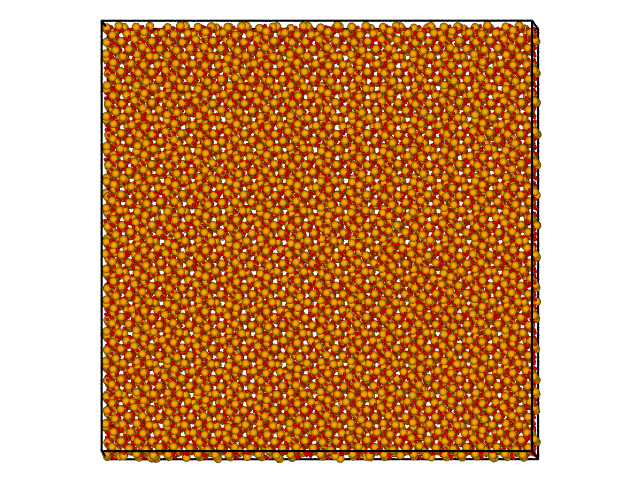
\includegraphics[width=0.24\textwidth]{graphics/initial_atoms.png}
    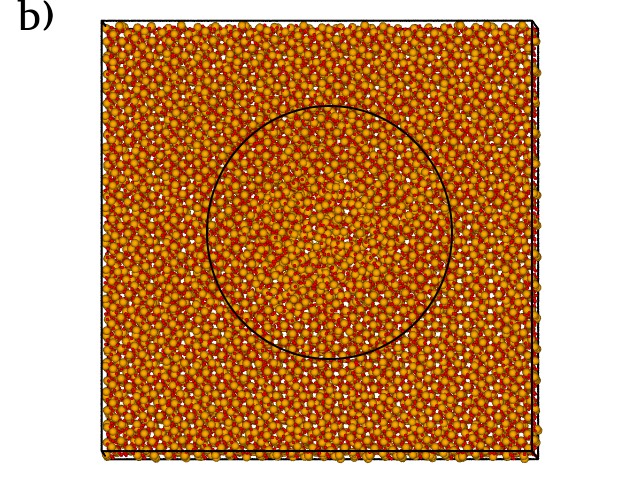
\includegraphics[width=0.24\textwidth]{graphics/spike_atoms.png}
    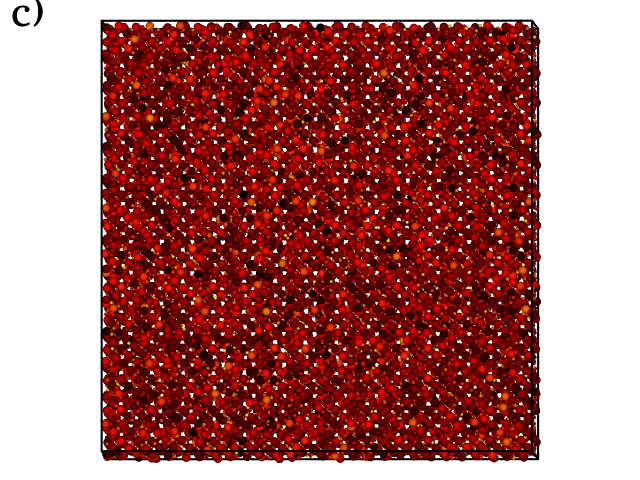
\includegraphics[width=0.24\textwidth]{graphics/initial.png}
    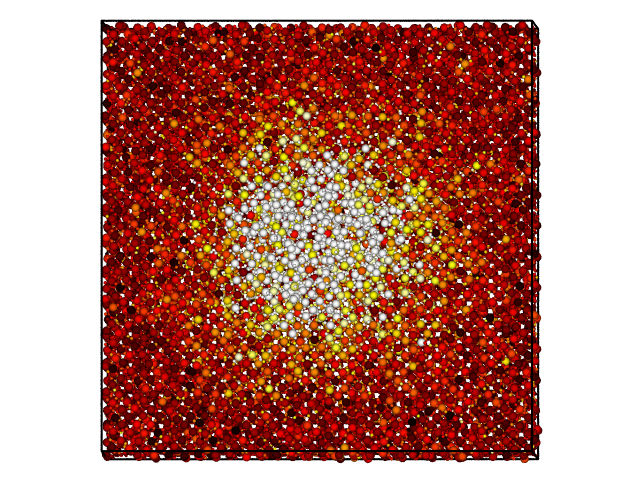
\includegraphics[width=0.24\textwidth]{graphics/spike.png}
  \end{center}
  \caption{Thermal Spike in SiO2}
\end{wrapfigure}

Previous studies have looked at the fine structure of SHI tracks (the narrow trails of permanent atomic distortion along penetrating SHI pathways) in thin film amorphous silica using small angle x-ray scattering (SAXS) measurements combine with non-equilibrium MD modeling and simulation techniques. These studies have successfully revealed that SHI tracks form a low density shell around the SHI path of penetration surrounded by an outer shell higher in density. The non-equlibrium MD calculations were carried out using an ~20k atom system where the track was produced by using the simple approach of instantaneous heating of  the atoms in the simulation cell along the SHI track path. This method has been motivated by the fact that most of the energy transfer from the electronic system to the atomic degrees of freedom occurs on the femtoseconds timescale.  The timescale of ionic displacements is much greater, implying the transfer is immediate. 

We intend to carry out similar simulations of comparable size that can be used to elucidate the structural changes observed in neutron scattering experiments of the average and local structure of these polymorphs of silica. Atomistic configurations from the end of this trajectory can then be fed into the RMC modeling to optimize the structure against the experimental data. The results of this study can help understand the fundamental degradation of silica materials exposed radiation damage and also to future work to manipulate nanoclusters within solid silica materials. 

An extension of this project would be to incorporate recently models that have been developed to address more realistic modeling of the electronic heat conduction to the atomic degrees of freedom. In these models, the solution of the electronic heat conduction is embedded into the MD simulations via including an electronic continuum used to solve a heat equation for modeling the energy transport between the atomic and electronic subsystems. The two-temperature model formalism of including the electron-phonon coupling has been previously used in modeling and simulating SHI bombardment of alpha-quartz, laser ablation, and shock simulations. Interestingly to our ICE-MAN project, this extension would allow us to bridge a quantum-to-molecular multiscale-modeling barrier. An important input parameter into the two-temperature model is the electronic specific heat. Recently, it has been shown that the electronic temperature depedence of the electronic specific heat can have an effect on the morphology of the SHI track that is formed.  To produce this relation, one calculates the difference in internal energy with change in the electronic temperature using finite-temperature density functional theory. Previous work of others have used the popular opEn Source Package for Research in Electronic Structure, Simulation, and Optimization (Quantum ESPRESSO) and the Vienna ab initio simulation package (VASP) softwares with proven scalability. Thus, we hope to use this project as a proof-of-concept workflow for ICE-MAN to: begin with quantum calculations, use outputs of these calculations as inputs into non-equilibrium MD simulations, and then use the atomic configurations of outputs from these simulations as inputs into RMC modeling to optimize the atomic structures against neutron scattering data.

\subsubsection*{Project 2: Modeling of amorphous germanium and silicon to determine high-pressure phase transformations}\label{haberl}

The second project is determining different structural changes of high-pressure amorphous germanium (a-Ge) and silicon (a-Si) from different forms of compression or indentation loads that result in new materials for industry applications \cite{Haberl2009, Borisenko2012, Haberl2014}. Similar to our first project, we will be modeling systems based on silicon that have been probed via neutron scattering carried out under high-pressure, being compressed in diamond anvil cells or being indented using diamond tips. These experiments were carried out at the Spallation Neutron and Pressure Diffractometer (SNAP) \cite{SNAPwebsite} at the SNS. Upon releasing the pressure load, these samples do not return to their initial state but stay in a different, metastable state. Based on either indentation or compression, improved electronic and photovoltaic properties have been observed in these materials. Also, high-pressure processing methods from this study could provide cheaper manufacturing methods for electronics \cite{Holmstrom2016}.

We will determine atomistic models that best fit neutron scattering experiments probing the average and local atomic structure via diffraction and pair distribution functions from experiments on both SNAP and NOMAD, along with vibrational density of states from vibrational spectroscopy carried out on the VISION neutron vibrational spectrometer instrument \cite{VISIONwebsite} at the SNS. To create models of a-Ge and a-Si in agreement with a large range of experimental data is still a current research challenge, and to date no such model exists. We have developed a structural relaxation program based on the Wooten-Winer-Weaire (WWW) method \cite{Wooten1985} to produce amorphized structures of a-Ge and a-Si via the Atomic Simulation Environment (ASE) \cite{ Bahn2002, ASEwebsite} from initially crystalline structures. Using this technique, we get amorphous structures that retain their four-fold coordination and bond-angle deviations in qualitative agreement with experiments\cite{Wooten1985}.  Equilibrium MD simulations can be used to further relax structures and non-equilibrium MD simulations can be used to replicate different experimental pressure loading and thermal annealing cycles. Atomic configurations from the MD trajectories are inputs into reverse RMC modeling to optimize the structure against the experimental data. Our hope that using ICE-MAN's unique capability of lowering the barrier for data cross-over from the MD simulations to the RMC optimization to fit to experimental data will allow a larger and faster search in the phase space and accelerate the convergence of a best fit to a variety of experimental data with strong emphasis on neutron data for these materials.
\subsubsection*{Project 3: Modeling oxygen insertion in one-dimensional channels of shafarzikite-like structures}\label{deLaune}
Support work in understanding the atomic-level structural changes in shafarzikite-like (FeSb2O4) structures. Will look specifically at the oxygen insertion into cobalt and lead doped derivatives of shafarzikite. These materials show promise in applications of electro-catalysis due to their unique 1-D cation channels with high peroxide anion mobility and potential for high, directed electronic conductivity. Will help with correction and analysis of the neutron scattering data to push modeling efforts to clarify the oxidized structures.



Propose the research projects that we can answer.  \\
  3) Sankar's project \\





\section*{Computational Methodology (applications/codes)}
\subsection*{LAMMPS}
The main engine for the MD simulations will be the Large-Scale Atomistic/Molecular Massively Parallel Simulator (LAMMPS) software. This code is highly-scalable for a variety of machine architectures: IBM BG/L, Cray XT3, Cray XT5, and Intel clusters with GPUs (Comet). It can take advantage of GPU and Intel MIC accelerators with good performance scaling. For documentation on general benchmarking of LAMMPS, the following website contains several benchmark problems for a variety of machines: \href{http://lammps.sandia.gov/bench.html}{http://lammps.sandia.gov/bench.html}. 


\subsection*{DFT Codes}
Currently, the VISION neutron vibrationl spectrometer instrument at the SNS has its own dedicated computer cluster, VirtuES, for carrying out  computer modeling as integral part of the neutron data analysis and interpretation of the spectra (discussed more in the Additional Comments). This cluster has a variety of DFT codes installed for carrying out eletronic struturce calculations to determine vibrational density of states spectra. Vision Users have a suite of codes to choose from: VASP, Quantum ESPRESSO, CASTEP, ABINIT, CP2K, RMG-DFT, and GULP. Also, the O'Climax software is currently being developed by the VISION team as software that can generate calculated incoherent INS spectra from the output of these listed DFT codes. 

A major thrust of the ICE-MAN project is to have an interface to the O'Climax code within the first year of the project. This implies that ICE-MAN will also interface with these DFT codes to create the workflow between these codes and eventually feed in to the structural modeling. A subset of these codes will be used for our quantum calculation work so explicit scaling and performance measurements are not show. We will only present a small test case for the Quantum ESPRESSO code only for the schafarzikite project.

\subsection*{RMCProfile}
The majority of fitting to neutron scattering data will be carried out using the RMCProfile \cite{Tucker2007, RMCProfileWebsite} software to perform reverse Monte Carlo optimization modeling. This software is able to fit many data types simultaneously (Neutron and X-ray total scattering, Bragg diffraction profiles, EXAFS, and single crystal diffuse scattering) and use a range of constraints to produce atomic models that are consistent with all the available data. The fitting will be carried out in a "perfectly parallel" (or "embarrassingly parallel") manner where an array of fits will be carried out simultaneously on serial processors with no communication between the processes. This makes the Open Science Grid XSEDE resource optimal to carry out the fitting optimization. The ICE-MAN project is an extension of the ICE project \cite{ICEwebsite}, which is already able to handle the launching and monitoring of local and remote jobs, visualizing and analyzing data, and managing data transfers. Thus, we will work towards automating a seamless transition from taking data located on an HPC resource generated by atomistic modeling and simulation and transferring it to the High Throughput Computing (HTC) resource where it will automatically be launched for fitting optimization, preserving HPC service units for jobs that can make use of the resource. This project would provide an impetus to push parallelization of the RMCProfile software to handle the large atomistic configurations generated and make use of the HPC resources, reducing optimization timescales.



\subsection*{Comet}
Comet is the ideal resource for our research for the following reasons:

\begin{enumerate}
\item It provides a heterogenous research platform that is capabable of providing domain-specific, ideal architectures. The compute nodes are ideal for our large-scale atomistic simulations and the large memory nodes are ideal for our quatum calculation work. The GPU nodes are available to tackle very large problem sizes that make use of massive level of parallelization efficiently

\item We are targeting the Oak Ridge National Laboratory Leadership Computing Facility resources (i.e. Titan) to launch ICE-MAN. However, due to all nodes containing a GPU on Titan, we can only use the machine to its full potential for a subset of our project. Using Comet as the first target machine allows us access to the resources we will eventually use, broaden the scope of machines that ICE-MAN can utilize, and be accessible to a larger part of the research community.

\item Members of the team already have experience using Comet and have had publications as a direct result of the allocations awarded on the machine.

\item The Data Oasis Lustre parallel file system ensures plenty of scalable storage available for the jobs run on the machine.

\end{enumerate}

\subsection*{Open Science Grid}
The Open Science Grid would be an optimal resource to use for launching multple arrays of reverse Monte Carlo jobs in a high throughput manner for large spanning of the phase space. The ICE-MAN project could take advantage on its already-underlying remote job launching capabilities to transfer work to the appropriate computational resource.

\subsection*{Performance and Scaling}


\section*{Computational Research Plan}
We propose to complete the following work on Comet 



\section*{Justification for Service Units (SUs) Requested}

Table \ref{SU_table} summarizes the jusitification for the requested resources to begin our project. The resources are 

\begin{table}[H]
  \caption{Summary of requested service units for projects}\label{SU_table}
  \resizebox{\textwidth}{!}{%
  \begin{tabular}{cccccc}
  	\toprule
  	Table & Project & Machine & Program & Service-Units & Storage (GB)\\
  	\midrule
  	1 & Irradiated SiO2   & Comet/Oasis & LAMMPS & 300,000 & 500 \\
  	2 & High-pressure a-Ge/a-Si & Comet/Oasis & LAMMPS & 300,000 & 500\\
  	3 & Oxygen in FeSb2O4 & Comet/Oasis & QE & 100,000 & 500\\
  	4 & RMC modeling   & OSG & RMCProfile & 25,000 & 100 \\
  	\bottomrule
  \end{tabular}
  }
\end{table}

Like it?

\section*{Additional Comments}
Currently, there is a shared comuter cluster available for computations for the group, the Virtual Experiments  in Spectroscopy  with neutrons (VirtuES) cluster. This machine was made available in 2015 as a funded Laboratory Directed Research and Development project for the VISION neurton vibraional spectrometer at the SNS. The machine consists of 2500+ cores with nodes consisting of two 16-core Intel Xeon E5-2698 v3 running at 2.30GHz. VirtuES is dedicated to the VISION beamline, the first SNS instrument that has computer modeling as integral part of the neutron data analysis and interpretation of the spectra. This cluster mainly used for running DFT calculations to help in data analysis and interpretation of User's neutron data. Our current proposed projects and ICE-MAN development comes secondary to Users needs.

There is also an open-research cluster, called Analysis, available at the SNS for Users to analyze and visualize their data from neutron experiments. This cluster is mainly for accessing and reducing User's data and not suited for HPC applications. MTM has currently just finished using a initial startup allocation for 100,000 total SUs from a previous project on the two XSEDE HPC resources at the San Diegoe Supercomputer Center: Comet and Gordon (50,000 SUs each)


\bibliography{draft}
\bibliographystyle{jponew}


\end{document}
